\section{DDC Traffic Characterization}
\label{sec:workloads}
In this section, we explore the first question: characterizing the network traffic in disaggregated datacenters. We start by outlining the methodology used in our study (\S\ref{ssec:method1}). In \S\ref{ssec:flc}, we discuss the flow-level characteristics (flow size distribution, inter-arrival times, etc.). We then discuss network-level traffic characteristics in \S\ref{ssec:nlc}, including traffic volume, spatial and temporal distribution. We close the section with a discussion on how various design knobs from \S\ref{sec:summary} impact our observations regarding the flow-level and network-level characteristics of traffic in disaggregated datacenters (\S\ref{ssec:knobs}).

\subsection{Methodology}
\label{ssec:method1} 
To characterize the traffic in disaggregated datacenters, we set up a testbed comprising of $5$ Amazon EC2 \texttt{m3.2xlarge} machines running Amazon Linux, each having $16$ vCPU, $32$GB of main memory, $1$TB of magnetic disk drives and $1$Gbps links. The Amazon EC2 machines we used were Private network enabled, ensuring no interference with other machines in the cluster. For each of the applications in Table~\ref{tab:workloads}, we capture local and remote data access flows, both for memory and disk.

\paragraphb{Inter-machine communication in \pdis}
To compare the traffic in \dis against the traditional server-centric architecture, we first characterize the flows in existing datacenters. To achieve this, we run the applications atop the above cluster. We then use {\tt TCPdump}~\cite{tcpdump}, which gives us a packet-level log of inter-machine communication. The packet-level log is combined into a flow level log by combining on the five-tuple; this approach has the limitation that the source port id a given application uses for various connections will be distinct. This is largely true except in the case of memcached, which maintains a unique port number for each client-server pair --- in this special case we limit flow sizes to the known request size of 10KB.

\paragraphb{Local and remote memory accesses in \dis}
To capture remote memory accesses, we first logically partition the main memory into ``local cache'' and ``remote memory''; for reasons described later, we use $30\%$ of the main memory as local cache. We then use an in-house implementation of a light-weight special instrumentation tool (SIT), implemented as a shim layer between the CPU and the swap device. The SIT intercepts all memory access requests into the part of main memory identified as remote. Since memory reads are assumed to be at the page granularity, all such captured requests have the same size (4KB). \rqc{SIT also captures the request time for each request, and ...} 

\paragraphb{Disk accesses in \dis}
We capture disk accesses during application runtime using the {\tt blktrace} utility, which provides disk access traces at the granularity of disk block sizes. Note that the data residing on a single disk is not necessarily on consecutive disk blocks (due to disk fragmentation); thus, a single file access from the disk may result in accessing non-consecutive disk blocks. Since {\tt blktrace} provides disk access patterns at the disk block granularity, it is impossible to infer which disk block accesses correspond to a single disk access request at the application layer. We, thus, use a simple heuristic to combine multiple disk block access into a single application layer request --- all those disk block accesses that occur within a small $\delta$ time range are combined into a single disk access. We study the sensitivity of our results against $\delta$ during traffic characterization. \rc{$\gets$ this is incorrect; we have to describe the mapping of disk addresses to disaggregated disk blades.}

\paragraphb{Data placement in \dis}
\rqc{We should describe how we map the disks in \pdis to those in \dis, and say that this mapping is simply a design knob.}

\paragraphb{Transforming data accesses into network flows}
In a disaggregated datacenter, it is possible to combine flows from multiple requests from the same source into a single flow. However, this would require changes in the application, and possibly in network elements at the end hosts. To avoid such complications, we simply assume that each remote memory access and disk access constitutes a flow in disaggregated datacenter.

\paragraphb{Limitations}

%
\begin{figure}
  \centering
  \subfigure{
    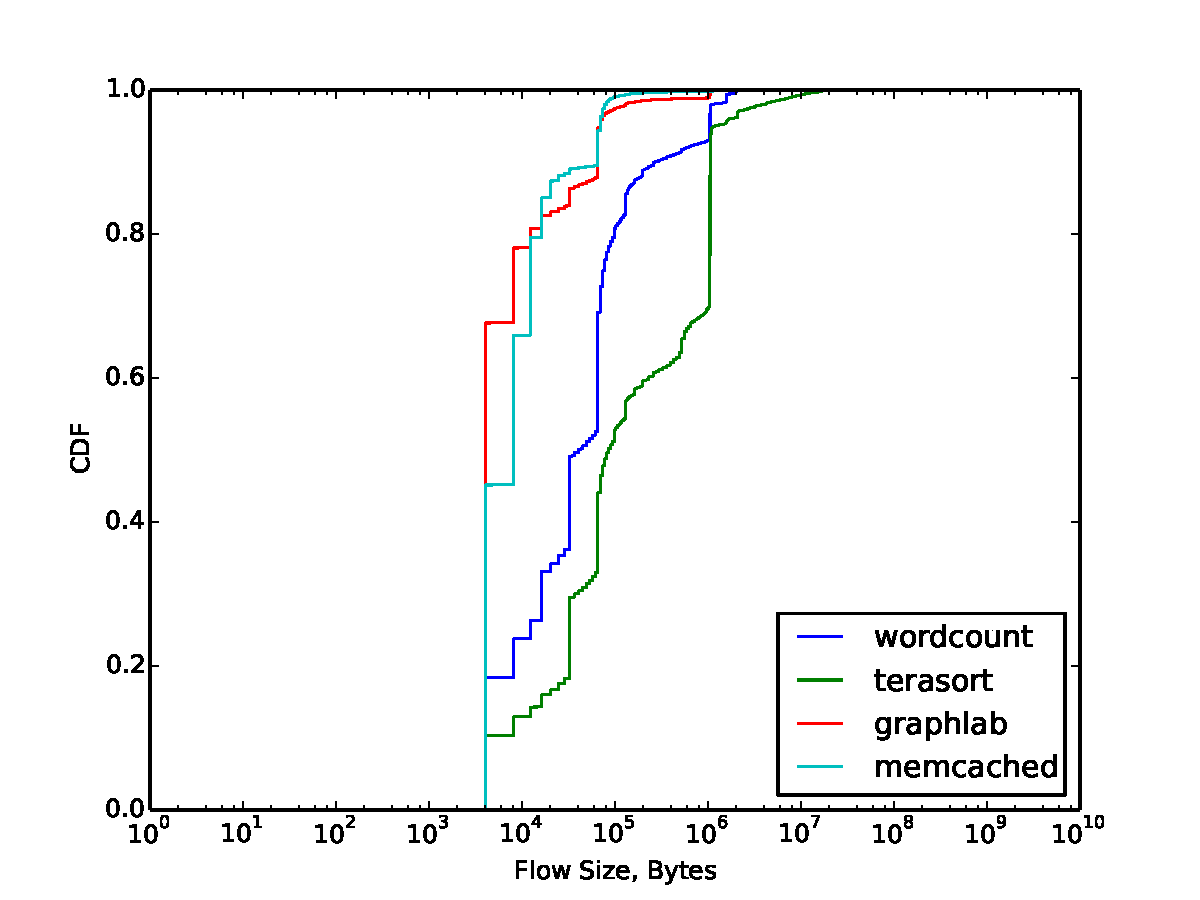
\includegraphics[width = 2.25in]{img/graph1_sizedist_dis} 
	\label{fig:asdd}
  }
%\hspace{0.05in}
  \subfigure{
    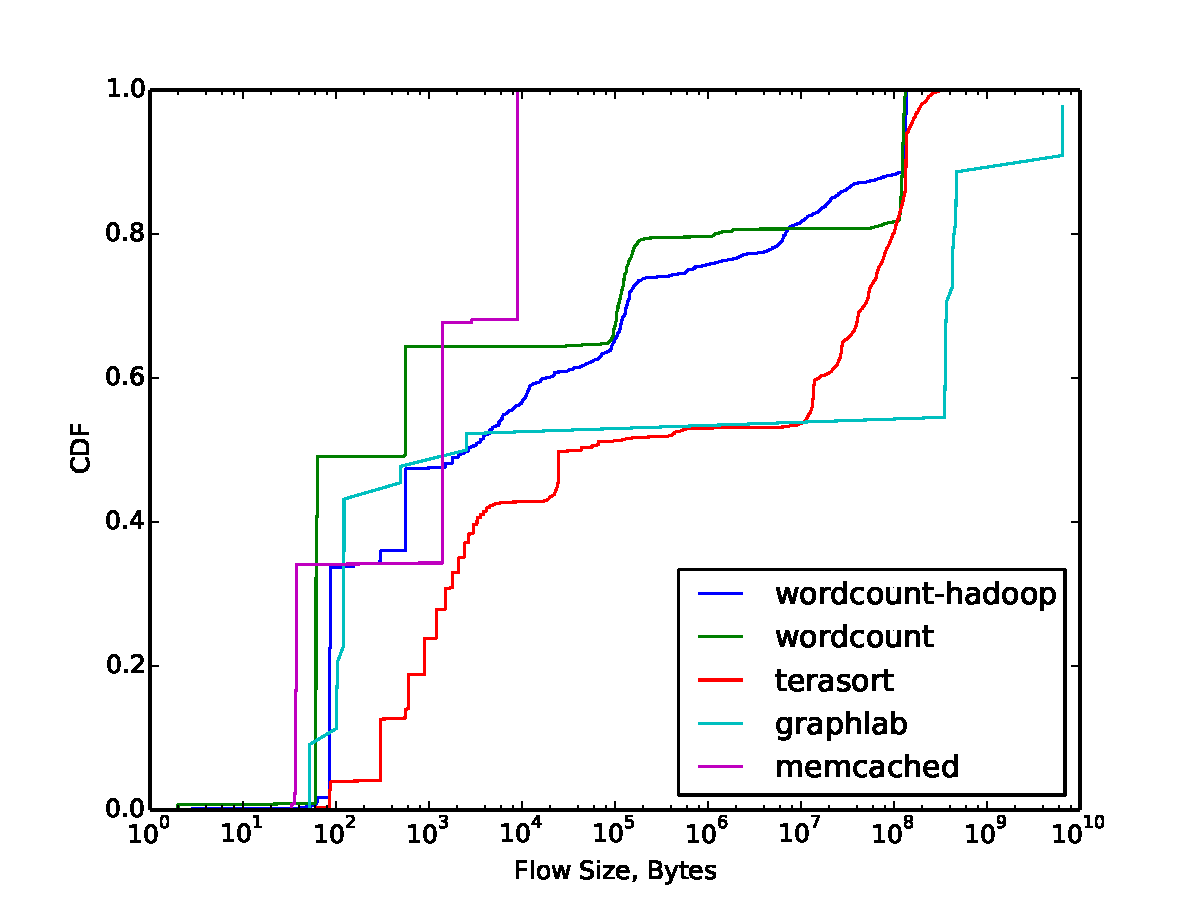
\includegraphics[width = 2.25in]{img/graph1_sizedist_pdis}
	\label{fig:sdds}
  }
  \caption{\small{\rqc{Flow size distribution in \dis (above) and \pdis (below). Note that the x-axis is log-scaled.}}}
  \label{fig:fsd}
\end{figure}
%

\subsection{Flow-level Characterization} 
\label{ssec:flc}
We start by discussing the flow-level characteristics in \dis, including flow size distribution, flow count and flow arrival time distribution. We then discuss some of the implications of our results regarding flow-level characterization of \dis traffic.

\subsubsection{Flow Size Distribution}
We start by discussing the flow size distribution in \dis. Figure~\ref{fig:fsd} shows the distribution of flow sizes across the six applications from Table~\ref{tab:workloads}. We make three interesting observations. First, the flow sizes are concentrated in the relatively small range [4KB, 40MB]. Second, across all the applications we evaluated, the flow size distribution is dominated by memory traffic (4KB flows) and at least $60\%$ of the flows are less than $100$KB. Finally, the tail in flow size distribution is almost non-existent, implying that irrespective of the application the elephant-mice effect typically observed in \pdis is absent.

Intuitively, the lack of short flows is because of \rc{$\gets$ I do not understand the reasons: here is a reason:} all inter-node traffic is at page granularity, and pages are 4KB long. Long flows are absent as a consequence of the data placement technique outlined in \S\ref{ssec:method1}. Overall, by enabling a more flexible placement of data, \dis \rc{will allow? Which tense we use will affect how people perceive the paper?} allows a more uniform distribution of flows injected into the network.

Figure~\ref{fig:fsd} also shows the flow size distribution with the same applications running atop \pdis. We note that the distributions are significantly different in \pdis --- the flow sizes span an additional two orders of magnitude both of short and on long flow sizes and the traffic is not dominated by any one particular flow size. Note that our flow size distribution in \pdis conforms with previous studies~\cite{imc-srikant, imc-theo}.

%
\begin{figure}
  \centering
    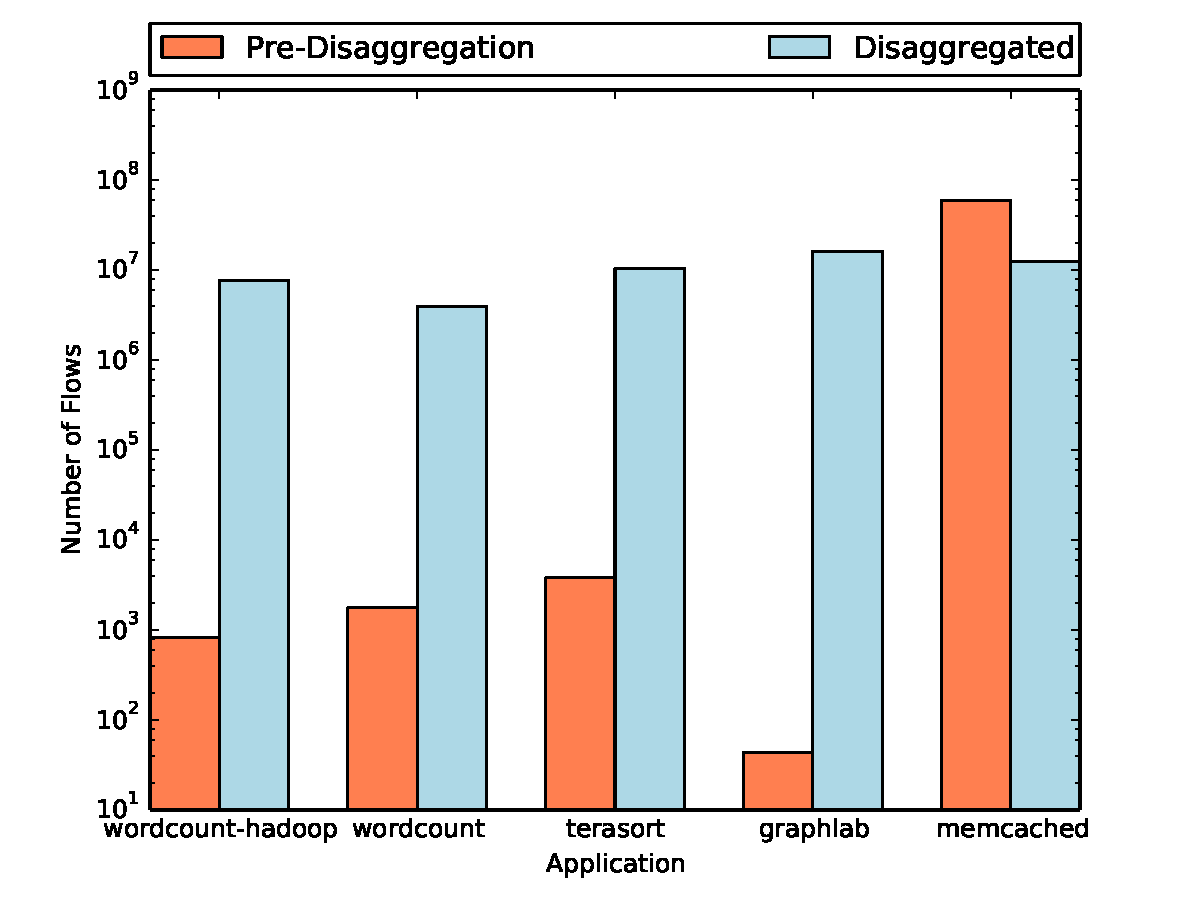
\includegraphics[width = 2.5in]{img/graph2_numflows} 
  \caption{\small{\rqc{Number of flows in \dis and \pdis. Note that the y-axis is log-scaled.}}}
  \label{fig:nof}
\end{figure}
%
%
\subsubsection{Flow count and volume}
\label{sssec:fctv}
Figure~\ref{fig:nof} shows that the number of flows in \dis increases by several orders of magnitude over \pdis for most applications. This is expected since a large number of disk and memory access flows that are contained within a server in \pdis (over PCIe, etc) are now injected into the network.

Interestingly, in memcached the number of flows in \ddc is fewer than in \pdis. After investigation, we found that while in \pdis each request will result in a network flow, in \dis some requests are serviced by the local memory cache without crossing the network. This phenomenon is discussed further in~\S\ref{sssec:tfvol}.

%Figure~\ref{fig:vof} shows that the number of bytes in \dis is more uniformly distributed across short and long flows when compared to \pdis. There are two main reasons for this -- the memory flows dominating the network flows (thus having more bytes in short flows), and the long flows having been distributed across the network leading to reduction in \#bytes in long flows \rc{$\gets$ not sure about this}
%
\begin{figure}
  \centering
  \subfigure{
    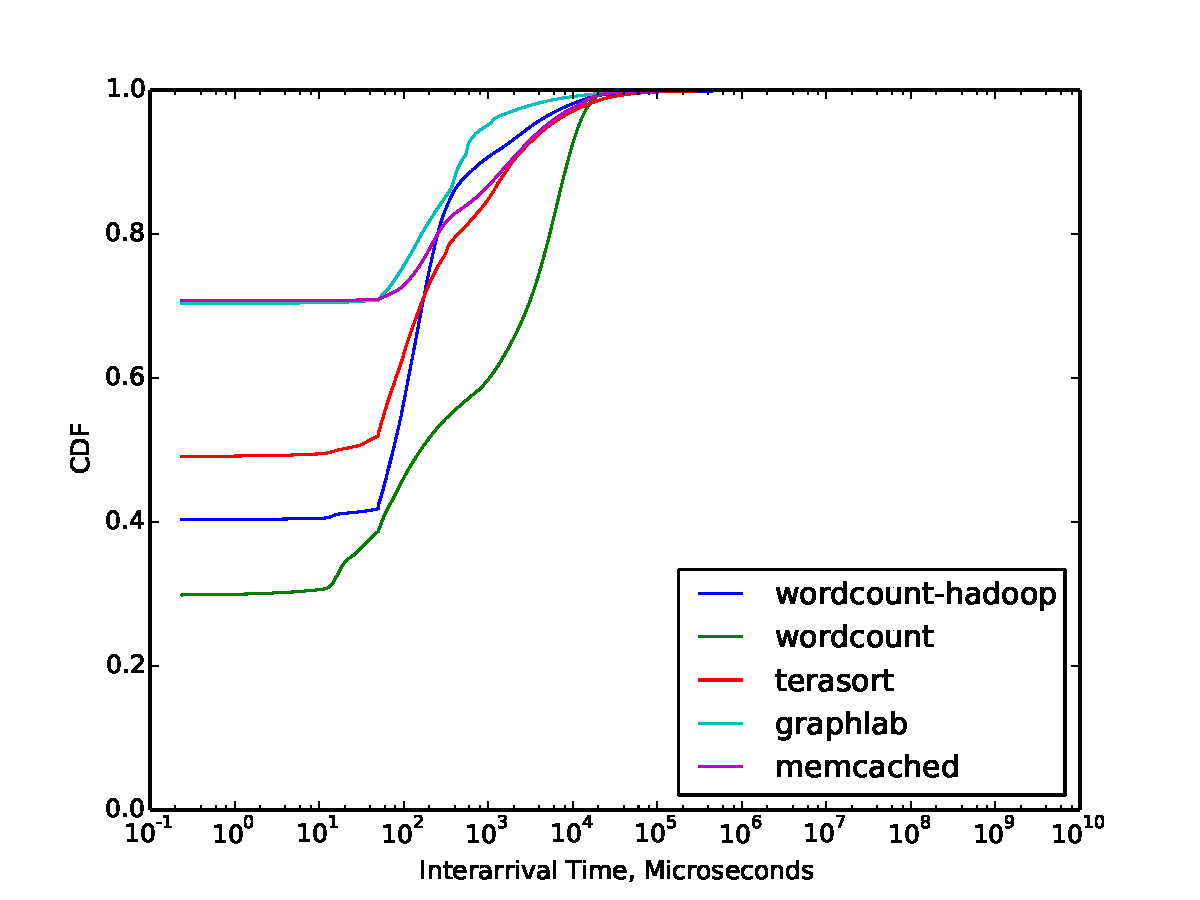
\includegraphics[width = 2.3in]{img/graph4_interdist_dis} 
	\label{fig:asdd}
  }
%\hspace{0.05in}
  \subfigure{
    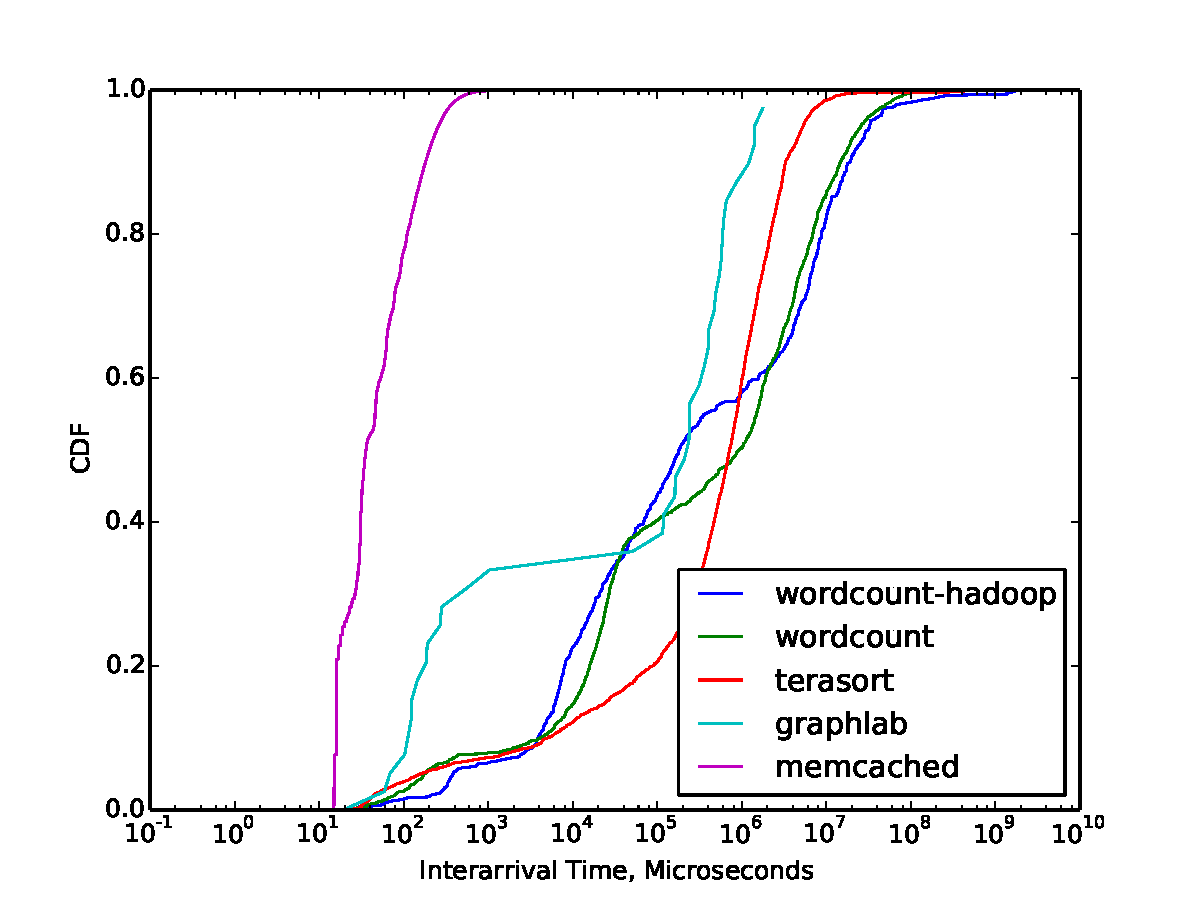
\includegraphics[width = 2.3in]{img/graph4_interdist_pdis}
	\label{fig:sdds}
  }
  \caption{\small{\rqc{Flow arrival time distribution in \dis and \pdis. All the applications go into one figure: six lines in the CDF, one for each application. The same thing for \pdis.}}}
  \label{fig:fat}
\end{figure}
%
\subsubsection{Flow Arrival Time Distribution}
\label{ssec:fatd}
\rc{This section along with figure 4 are slated for removal because we cannot count remote memory flows.}
Next, we study the flow arrival times in \dis. Figure~\ref{fig:fat} shows the flow arrival time distribution for the six applications from Table~\ref{tab:workloads}. We make two interesting observations. First, the flow arrival time distribution is essentially independent of the application. This is because memory access traffic dominates all the applications, leading to similar flow arrival time distribution. Second, the flow arrival time distribution is significantly different from Poisson distribution, a commonly accepted approximation to workloads in \pdis. \rc{We should say something about inter-flow arrival times --- too small? not too small? any significant different compared to \pdis?}

Figure~\ref{fig:fat} also shows the flow arrival time distribution in \pdis. As observed in several previous studies~\cite{imc-srikanth, imc-theo}, the distribution is very close to Poisson distribution providing a second order support to our evaluation methodology. In comparison to \pdis, the distribution is significantly different in \dis as discussed above.

\subsubsection{Implications}
\begin{itemize}[leftmargin=*]
	\itemsep0em
	\item Traffic dominated by latency-sensitive short flows --- centralized flow schedulers may be inefficient
	\item Number of flows increased --- centralized solutions may see more scalability issues
	\item \rc{slated for removal} Flow arrival times too small --- centralized solutions inefficient
	\item More homogeneity in flow sizes --- design of protocols
	\item \rc{remove?} Traffic volume more uniformly distributed across short and long flows --- ??
\end{itemize}

\subsection{Network-level Characterization} 
\label{ssec:nlc}
We now study the network-level characteristics in \dis, including network traffic volume, spatial distribution and temporal distribution. We then discuss implications of our study of network-level characterization of \dis traffic.

%
\begin{figure}
  \centering
    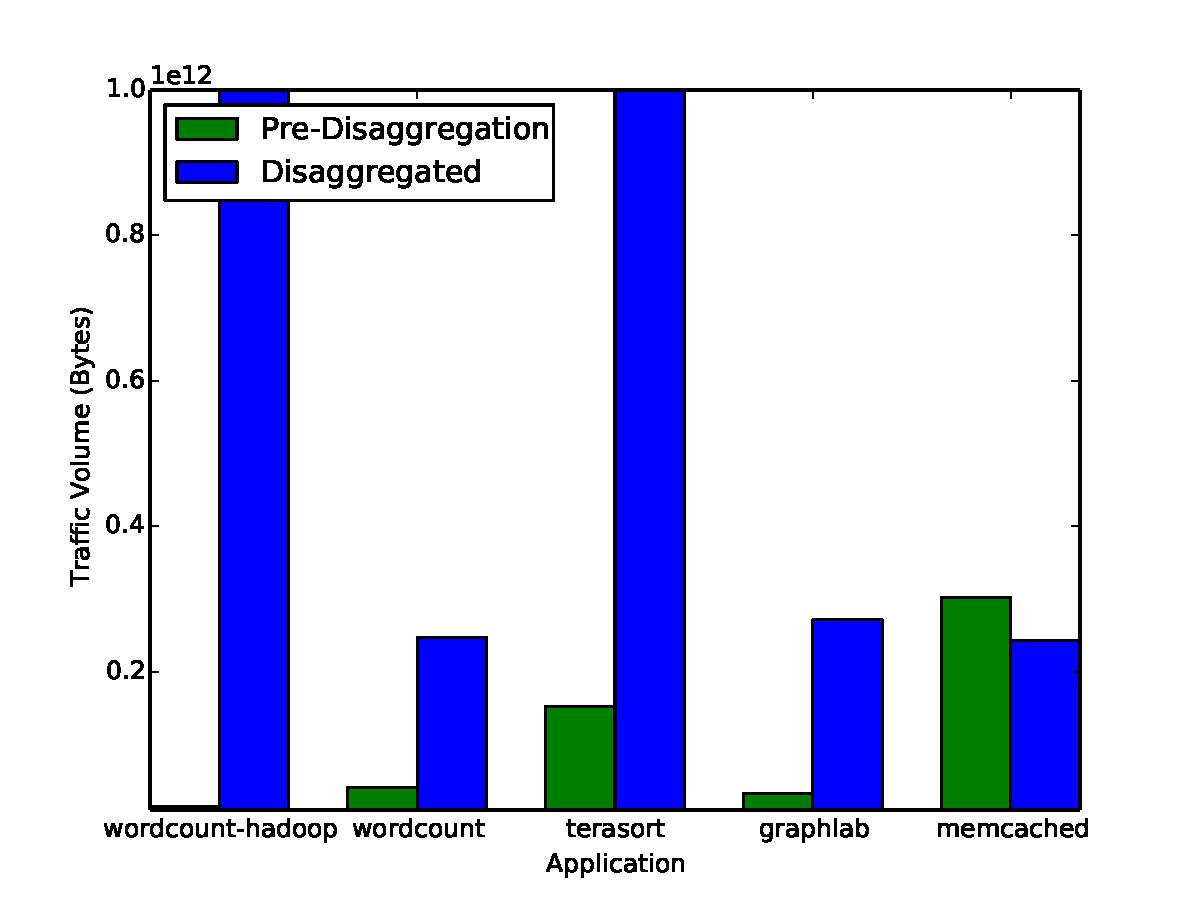
\includegraphics[width = 2.5in]{img/graph5_trafficvolume} 
  \caption{\small{\rqc{Traffic volume in \dis and \pdis.}}}
  \label{fig:vol}
\end{figure}
%
\subsubsection{Traffic volume}
\label{sssec:tfvol}
We start with studying the traffic volume in \dis and \pdis (see Figure~\ref{fig:vol}). For most applications studied, the traffic volume in \dis increases due to the same reason the number of flows increases (shown in Figure~\ref{fig:nof}) --- flows that previously were contained within a server are now carried over the network.

Wordcount demonstrates an especially drastic increase in traffic volume in \dis. \rc{The reason why wordcount has more flows}

Just as memcached exhibits a greater number of flows in \pdis, its traffic volume is greater in \dis. Our experiments with 25\% of memory in the local cache, so we expect that approximately this amount of request traffic in memcached will be served from the local cache in \dis and avoid the network entirely. Accordingly, we observe that the difference in traffic volume between \dis and \pdis is 24\%. The difference in the number of flows is more drastic because the flow distributions are different --- while memcached in \pdis has a bimodal distribution of request and response flows of approximate size 30 bytes and 10KB respectively, in \dis the distribution varies in the range [4KB, 19MB]. The longer tail in flow sizes for \dis causes the drastic disparity in number of flows seen in Figure~\ref{fig:nof} despite a relatively modest increase in traffic volume.

% We note that the traffic volume in \dis is not much larger than in \pdis. At the first glance, this may seem rather surprising given the increase in traffic due to intra-server traffic becoming remote. However, note that memory accesses are just $4$KB in size; thus, a significantly large number of memory access traffic will correspond to a single long flow. Moreover, reads and writes that are local are only increased by a factor of $2\times$.

%
\begin{figure}
  \centering
  \subfigure{
    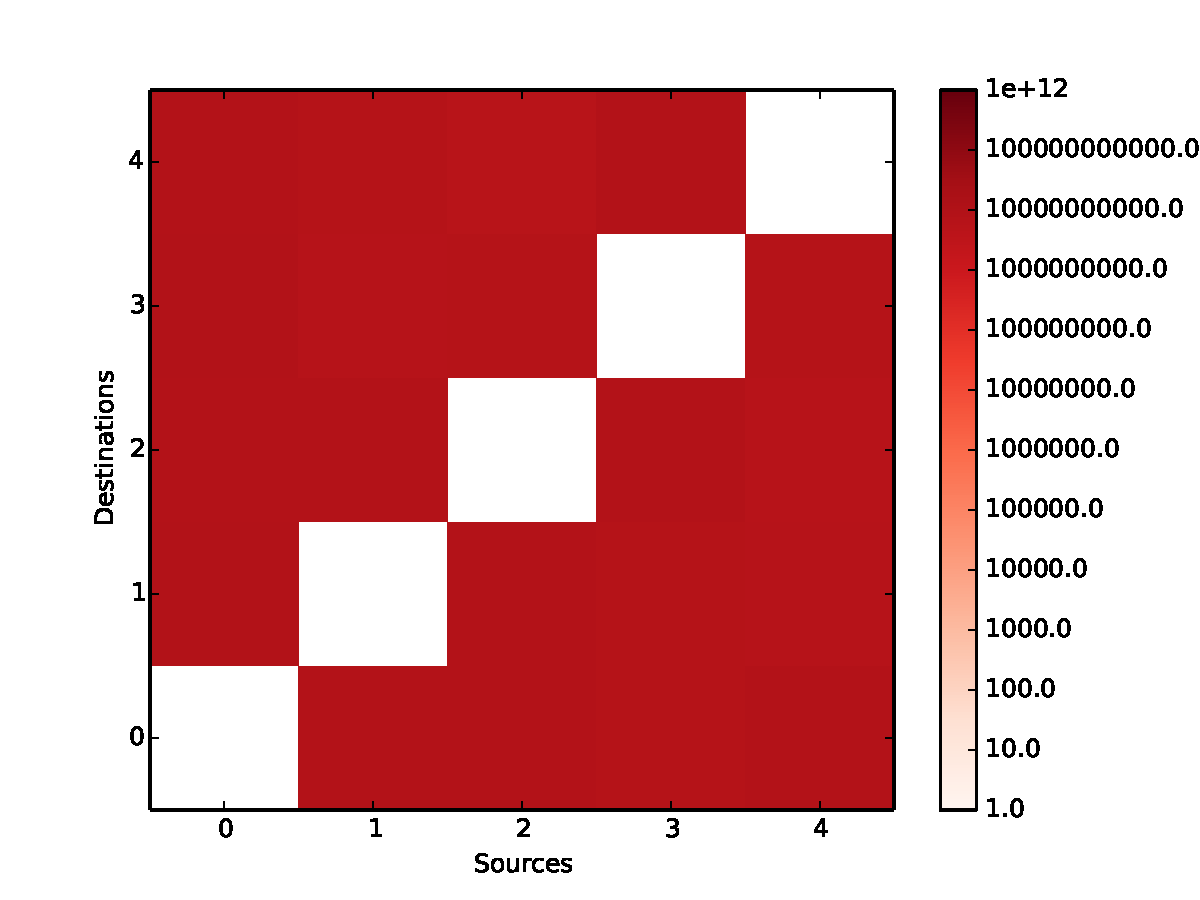
\includegraphics[width = 2.3in]{img/graph6_trafficvolumeheatmap_pdis_terasort} 
	\label{fig:asdd}
  }
%\hspace{0.05in}
  \subfigure{
    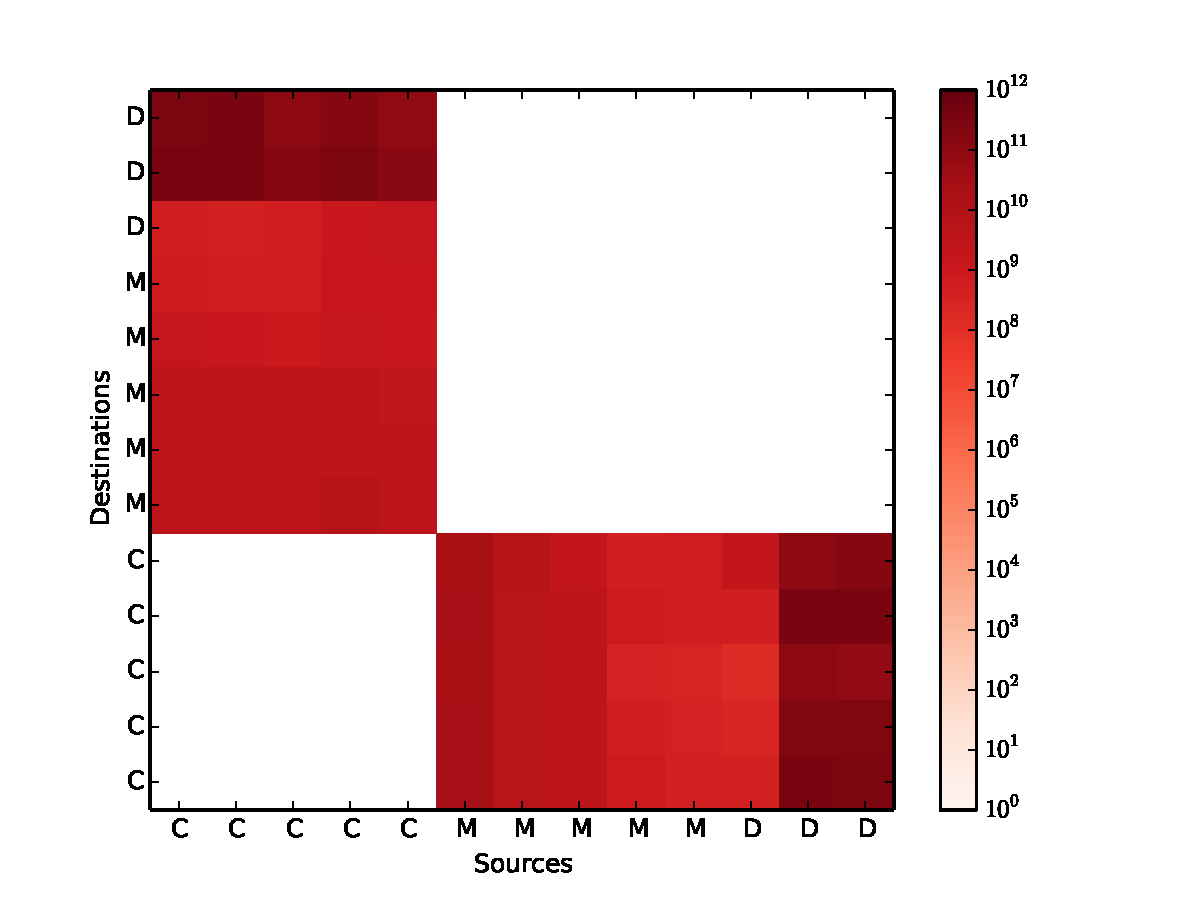
\includegraphics[width = 2.3in]{img/graph6_trafficvolumeheatmap_dis_terasort}
	\label{fig:sdds}
  }
  \caption{\small{\rqc{Spatial traffic distribution in \dis and \pdis. The x-axis represents senders and the y-axis receivers. In \pdis above, this is a $5 \times 5$ matrix for the 5 ec2 machines, while in \dis below, the heatmap is a $13 \times 13$ matrix, for the 5 cpu blades, 5 memory blades, and 3 disk blades we map the 5 ec2 machines to. For further details on this mapping see \S\ref{ssec:method1}. Blue means less traffic and red means more.}}}
  
  %A $n \times n$ matrix heat diagram, with cell $(i, j)$ having heat level corresponding to the traffic volume between source i and destination j. The same thing for \pdis.}}}
  \label{fig:sd}
\end{figure}
%
\subsubsection{Spatial distribution}
We now study the spatial distribution of traffic in \dis (see Figure~\ref{fig:sd}). We make two observations. First, \rc{something}. Second, the overall spatial distribution in \dis has significantly lower temperature than in \pdis, implying that on an average, each source-destination pair observes significantly lower traffic volume in \dis when compared to \pdis.

%First, when compared to \pdis, the traffic in \dis is significantly well distributed across the source-destination pairs. Indeed, the \dis architecture allows distributing a single read/write traffic across multiple nodes spatially distributed across the network. Second, the overall spatial distribution in \dis has significantly lower temperature than in \pdis, implying that on an average, each source-destination pair observes significantly lower traffic volume in \dis when compared to \pdis.

\subsubsection{Temporal distribution}
Finally, we study the temporal distribution of traffic in \dis and \pdis. Figure~\ref{fig:td} shows that, when compared to \pdis, the traffic distribution in \dis is significantly less bursty. This is because of an interesting effect caused by the data placement discussed in \S\ref{sec:summary}. When a long flow in \pdis is divided across multiple smaller flows in \dis (due to data placement across multiple disks), it is pipelined into multiple shorter flows. Akin to the task packing problem, where having multiple smaller tasks has a better packing compared to a single long task, dividing a single flow into multiple smaller flows ``packs'' into the network more efficiently, making traffic less bursty.
%
\begin{figure}
  \centering
  \subfigure{
    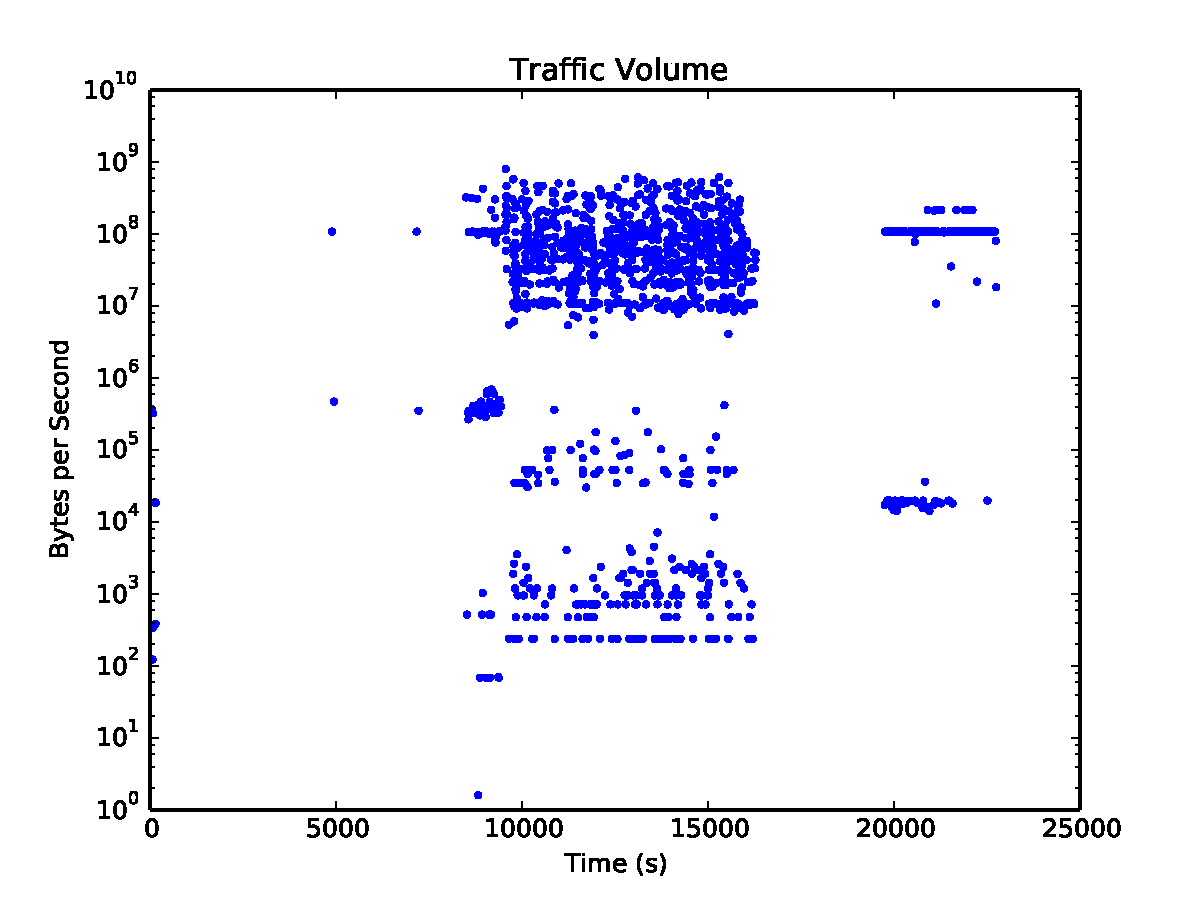
\includegraphics[width = 2.3in]{img/graph7_temporaltraffic_pdis_terasort} 
	\label{fig:asdd}
  }
%\hspace{0.05in}
  \subfigure{
    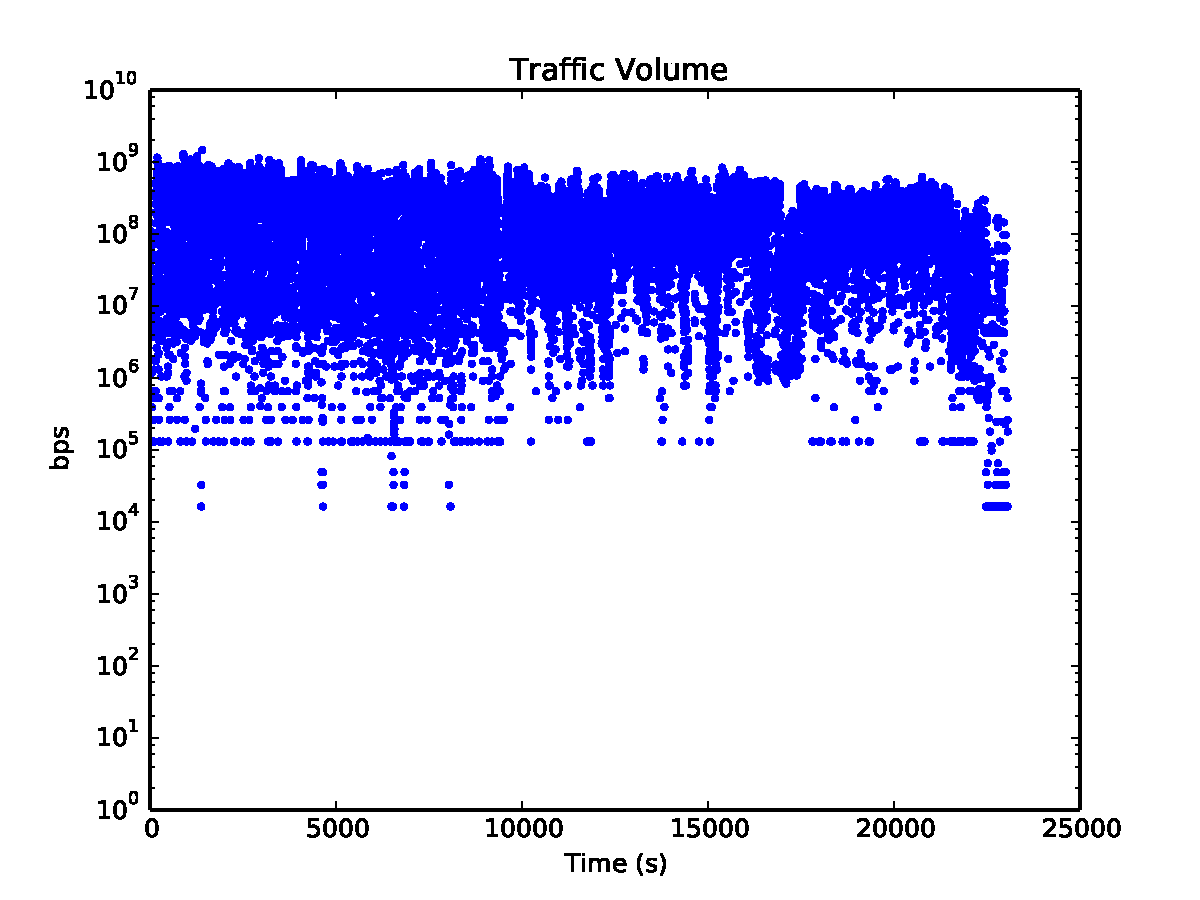
\includegraphics[width = 2.3in]{img/graph7_temporaltraffic_dis_terasort}
	\label{fig:sdds}
  }
  \caption{\small{\rqc{Temporal traffic distribution in \dis and \pdis for one of the applications. The trace was divided into 100ms timeslots, and flows were assigned to slots based on their start time. The traffic volume in these timeslots was then normalized to determine a value in bytes per second. Note the y-axis is log-scale.}}}
  \label{fig:td}
\end{figure}
%

\subsubsection{Implications}
\label{ssec:implications}

\begin{itemize}[leftmargin=*]
	\itemsep0em
	\item Traffic volume --- do not need very high bandwidth networks
	\item Spatial distribution --- traffic not so local
	\item Temporal distribution --- do not need to design networks for peak traffic?
\end{itemize}		

\subsection{Impact of design knobs}
\label{ssec:knobs}
We now study how various design parameters in \dis architecture design impact the observations made in this section. 

\paragraphb{Impact of cache size}

\paragraphb{Impact of disaggregation scale}

\paragraphb{Impact of data placement}

\paragraphb{Impact of remote versus local}